\chapter{Future directions}
\label{chap6}


Closing chapter 

\section{Introduction}
More blaa


There is mounting evidence that aspartate limitation effects nucleotide metabolism.
Increased cell size, Chk1/2 phosphorylation, increase/decrease in NTP/dNTPs.
This is hard to rescue/investigate because ...

Cell size the nucleotide imbalance hypothesis.
%%% See "ETCrescue" folder under lab-work

Gln depletion causes cells stuck in S-phase due to Asp depletion \cite{Patel2016-ms}.




\begin{figure}
    \centering
    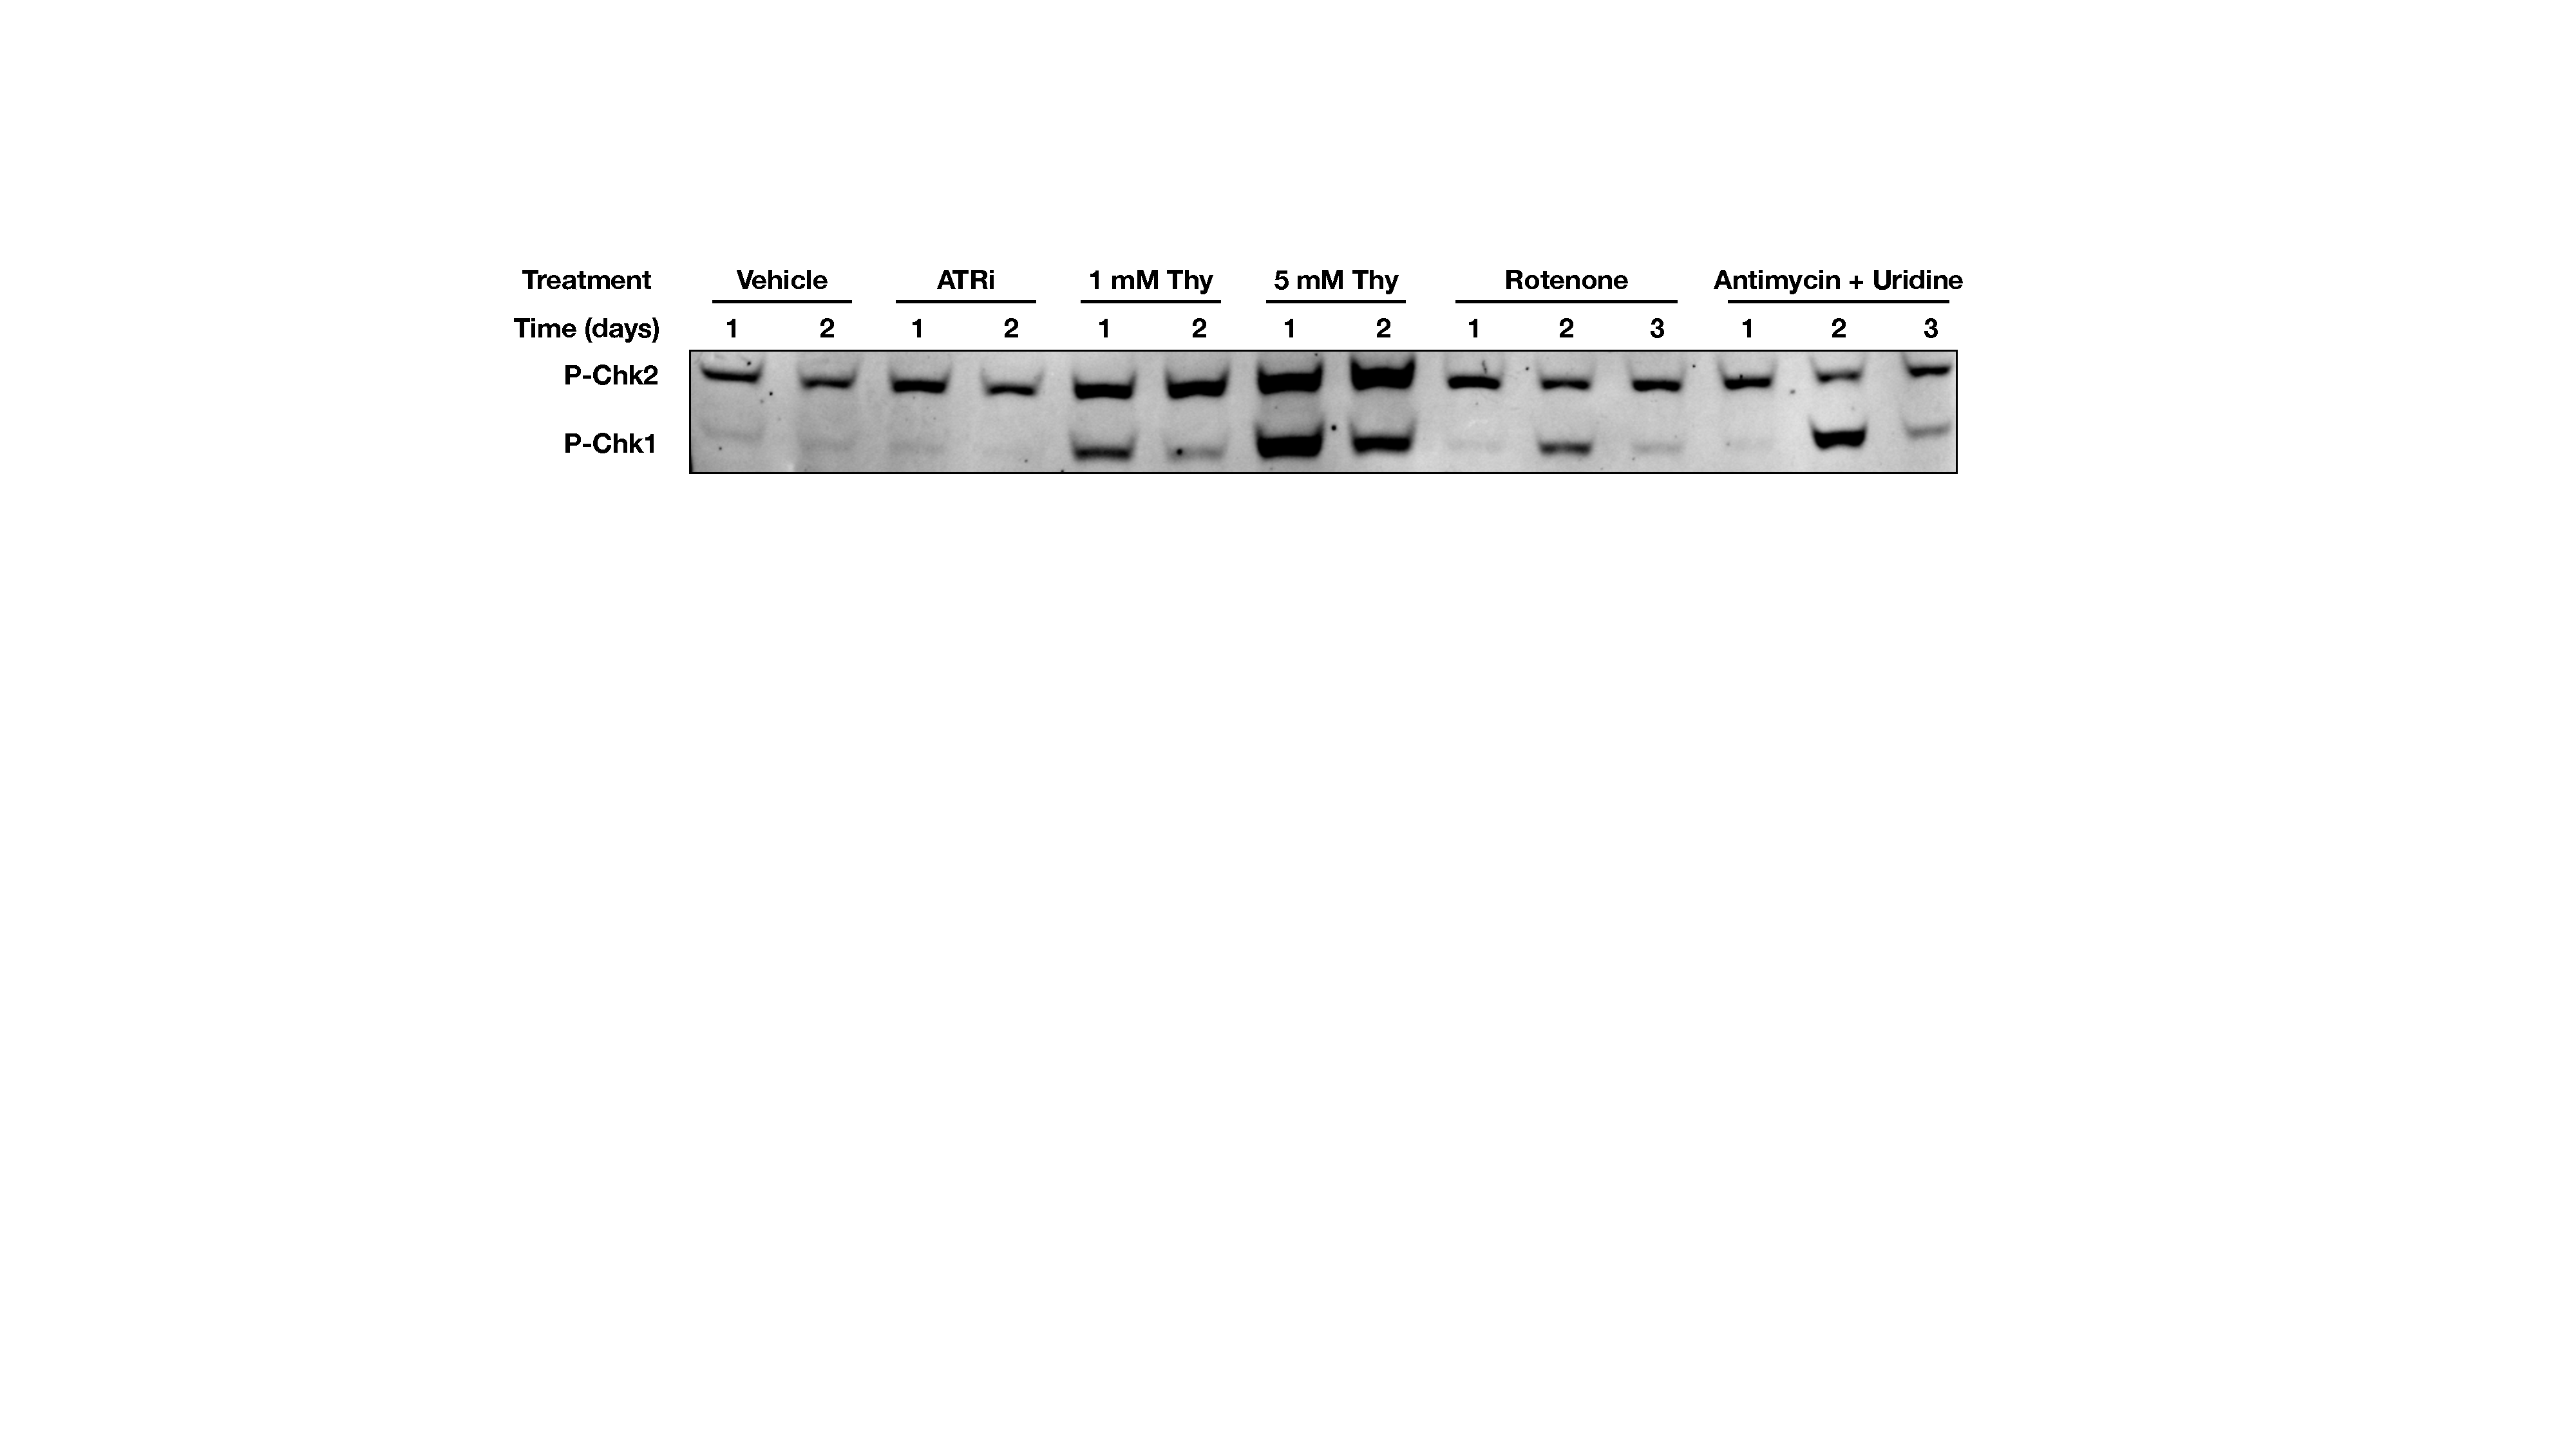
\includegraphics[width=0.85\textwidth]{figures/chap6/P_Chk_wstrn.pdf}
    \caption[gggg]{
    gggg
    }
    \label{fig:ch6:P_Chk_wstrn}
\end{figure}



Hadacidin (Asp analog) suppresses ATP synthesis by inhibiting adenylosuccinate synthetase at a dose lower than necessary to inhibit pyrimidine or protein synthesis \cite{Shigeura1962-nu, Shigeura1962-ot}.

Hadacidin decreases ATP and increases GTP while mycophenolic acid decrease GTP only in Ehrlich ascites tumors \cite{Barankiewicz2011-ak}

Hadacidin is toxic to cells and its potency is amplified by aspartate limitation induced by phenformin.
Phenformin amplification is reversed by pyruvate, alpha-ketobutyrate and aspartate.
Adenine reversed hadacidin toxicity while neither neither asparagine nor uridine had any effect indicating that adenylosuccinate synthetase inhibition is the primary target of hadacidin \cite{Neuman1963-dx}.

Hadacidin inhibited proliferation, increased cell size and arrested cells in S phase of the cell cycle \cite{Ladino1989-rj}.

Hadacidin had no useful clinical effect as a chemotherapy [Cancer chemotherapy reports 1968].




Other trends within cancer metabolism include increased glutamine consumption and dependence [refs],
serine metabolism [refs]
folate metabolism [refs]
aspartate metabolism [refs]
redox metabolism [refs]

The therapeutic success of targeting cancer metabolism has been underwhelming.
Many attempts to target lactate fermentation through inhibition of the lactate transporters, lactate dehydrogenase, the glucose transporters or essential steps in glycolysis has failed.

[refs] with some exceptions (ASNase, IDH, others?) but remains an active area of research.

There are many reasons why targeting cancer metabolism has failed, one reasons is the simple fact that there is little metabolic difference between cancer cells and non-cancerous rapidly proliferating cells.
As such targeting cancer metabolism may equally target proliferating cells and thus were merely be a new form of chemotherapy.
But alas, the Ahabian search for the white whale continues.






\begin{figure}
     \centering
     \begin{subfigure}[b]{0.49\textwidth}
         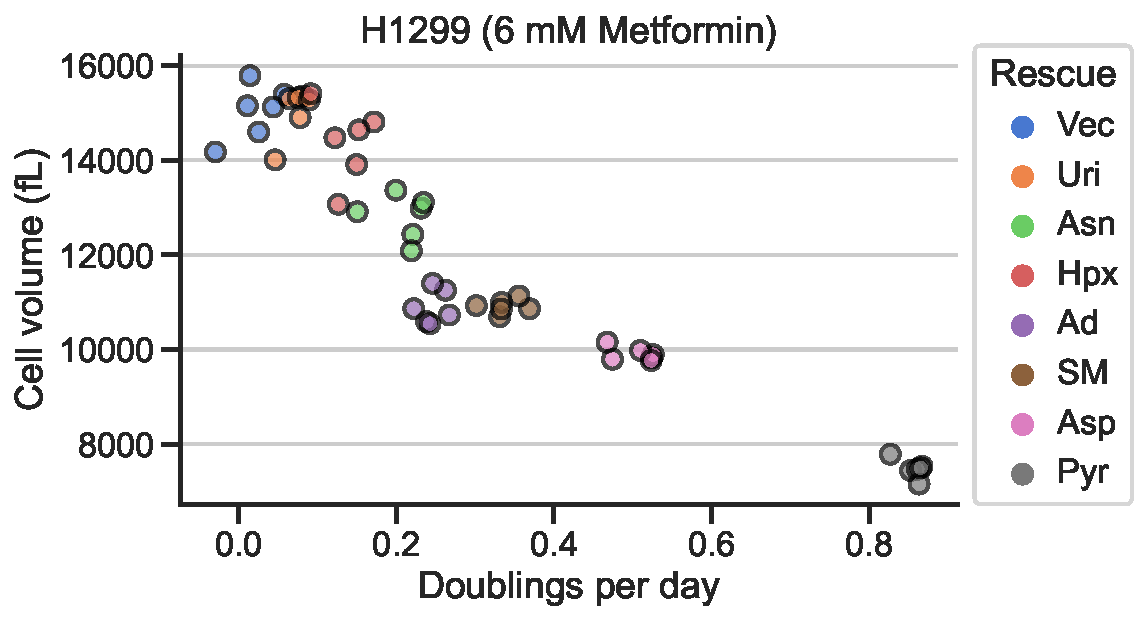
\includegraphics[width=\textwidth]{figures/chap6/H1299_Met_cellvol.pdf}
         \caption{}
         \label{fig:ch6:H1299_Met_cellvol}
     \end{subfigure}
     \hfill
     \begin{subfigure}[b]{0.49\textwidth}
         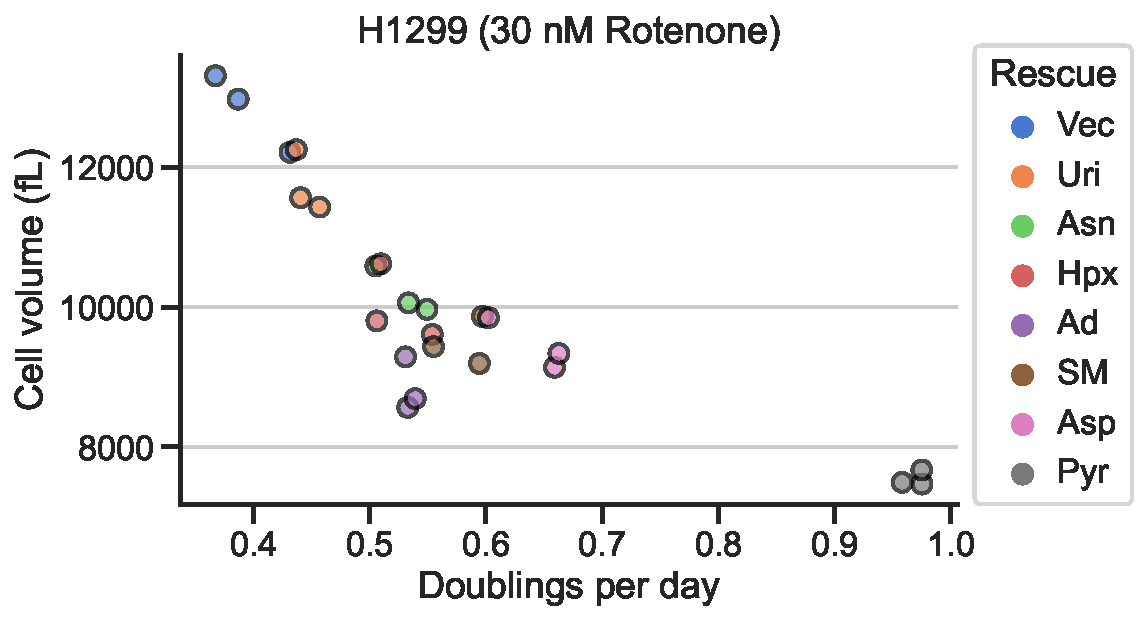
\includegraphics[width=\textwidth]{figures/chap6/H1299_Rot_cellvol.pdf}
         \caption{}
         \label{fig:ch6:H1299_Rot_cellvol}
     \end{subfigure}
        \caption[hhhh]{
        Cell volumes in (a) and (b) from endpoint counts from figures \ref{fig:ch2:H1299_Met_rescue} and \ref{fig:ch2:H1299_Rot_rescue}, respectively.
        }
        \label{fig:ch6:H1299_ETCrescue_vol}
\end{figure}










% Cell signal	2348T	Phospho-Chk1 (Ser345) (133D3) Rabbit mAb #2348
% Cell signal	2197T	Phospho-Chk2 (Thr68) (C13C1) Rabbit mAb #2197


Further use an development of the aspartate sensor.
Mito version
Coupled with screening (here it would be better to use laser microscope to "mark" the cells before sorting)


Development regarding the tRNAseq method.
There is a big opportunity to systematically test different RT polymerase to find ones with better readthrough.
Using cupric ions to increase speed of chemistry.
Integrate chemical treatment of RNA to expand the detection of RNA modifications.
Test and validate ways of increasing throughput e.g. ligation of whole cells RNA.
Internal control for RNA modification detection, maybe tRNA isolated from another organism (e.coli, or another bacteria with few tRNA transcripts.)
Expanding into animal tissue, first sampling all relevant tissues to get charge, expression and modifications at baseline, then applying it in disease states to detect any differences.
Expand its use for measuring relevant rates beyond charge half-life, e.g. tRNA charge kinetics on a library of tRNAs (see simulated data).






